\mychapter{Literature}{Literature}{}
\label{chap:literature}

\mysection{Introduction to review}{Introduction to Review}
\label{sec:lit_intro}

This chapter reviews the literature relevant to the design of a low-cost, high-performance potentiostat for \ac{DPV}. The purpose of this review is to establish the electrochemical and hardware fundamentals required to design such an instrument, and to survey the existing landscape of commercial and open-source potentiostat designs in order to identify a gap in the current market. The project's aim is the development of a low-cost potentiostat with improved performance and usability relative to existing open-source alternatives.

\mysection{Electrochemical background}{Electrochemical Background}
\label{sec:electrochemical_background}

\mysubsection{Basics of electrochemical cells}{Basics of Electrochemical Cells}
\label{sec:basics_electrochemical_cells}

A potentiostat controls the potential between the reference and working electrode while simultaneously measuring the current flowing between the counter and the working electrode. This is a popular three-electrode setup for measurement, illustrated in Figure~\ref{fig:three_electrode}. The \ac{WE} is the focal area of electrochemical reactions \cite{lodh2023}. In a three-electrode system the potential around it is measured and manipulated to study the desired catalyst or analyte, where an analyte is a specific substance or chemical component that is the subject of analysis.

The \ac{RE} provides a stable, known potential that is used as a benchmark to control and monitor the working electrode's potential \cite{cengiz2021}. Current flow through the reference electrode is minimal to ensure that its potential remains accurate \cite{cengiz2021}. The \ac{CE} (also called the auxiliary electrode) completes the circuit, allowing current to be sourced or sunk between it and the working electrode, which prevents the reference electrode from being affected \cite{cengiz2021}. The reaction at the counter electrode should be monitored, as corrosion at the electrode could interfere with measurement accuracy \cite{cui2023}. The three-electrode setup is the foundational hardware configuration for the voltammetric techniques that will be discussed later, namely \ac{CV}, \ac{LSV}, \ac{SWV}, \ac{DPV}, and stripping voltammetry.

\begin{figure}[H]
    \centering
    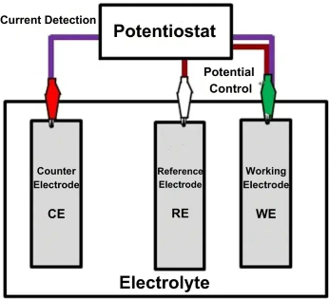
\includegraphics[width=0.6\linewidth]{figures/electrode.png}
    \caption{The three-electrode electrochemical cell configuration (working, reference and counter electrodes).}
    \label{fig:three_electrode}
\end{figure}

\mysubsection{Voltammetry as a family of techniques}{Voltammetry as a Family of Techniques (CV, LSV, SWV, DPV, Stripping Voltammetry)}
\label{sec:voltammetry_family}

In any voltammetric measurement, applying a voltage to an electrode generates two types of current:

\begin{itemize}
    \item \textbf{Faradaic current:} The actual current generated by the transfer of electrons during the oxidation or reduction of the target analyte \cite{alyamni2024}. This is the desired signal.
    \item \textbf{Charging (capacitive) current:} The background current generated simply by charging the electrical double-layer at the electrode surface, which acts like a capacitor caused by the Helmholtz plane \cite{alyamni2024}. This causes background noise.
\end{itemize}

The same three-electrode setup handles each of the following techniques in a different way:

\begin{itemize}
    \item \textbf{Linear Sweep (\ac{LSV}) and Cyclic Voltammetry (\ac{CV}):} The potentiostat applies a continuous, linear voltage ramp (or a triangular sweep for CV). The counter electrode continuously sinks or sources the resulting faradaic current.
    \item \textbf{Differential Pulse (\ac{DPV}) and Square Wave Voltammetry (\ac{SWV}):} Instead of a continuous ramp, the potentiostat applies a series of discrete voltage pulses or steps. By measuring the current at specific times during the pulse, the system can mathematically subtract the background capacitive (charging) current. This dramatically increases sensitivity, making DPV and SWV the preferred techniques for trace-level detection in biosensing applications.
    \item \textbf{Stripping voltammetry:} This is a two-step process that still relies on the exact same electrodes. First, the potentiostat holds a constant potential to electroplate (pre-concentrate) the analyte onto the working electrode. It then applies a sweep or pulse waveform (often an LSV, DPV, or SWV waveform) to ``strip'' the analyte back into the solution, yielding a large current spike.
\end{itemize}

\mysubsection{Differential pulse voltammetry theory}{Differential Pulse Voltammetry Theory}
\label{sec:dpv_theory}

\ac{DPV} superimposes small pulses of potential onto a linear potential ramp or staircase. The current difference is measured before and near the end of each pulse to reduce background charging current and achieve high sensitivity \cite{pineresearch_dpv}, although this comes at the cost of time resolution \cite{sciencedirect1993dpv}. DPV builds on the foundations of linear sweep methods; however, it uses a more complex, discontinuous voltage waveform.

\mysubsection{Waveform description}{Waveform Description (Pulse Height, Pulse Width, Step Potential, Current Sampling Windows)}
\label{sec:dpv_waveform}

In \ac{DPV}, the excitation waveform consists of a foundational staircase ramp with a discrete voltage pulse superimposed onto each step, as shown in Figure~\ref{fig:dpv_waveform}. The geometry of this waveform is defined by the pulse amplitude, which dictates the voltage magnitude of the superimposed pulse, and the pulse width, which specifies how long this elevated potential is held before the system returns to the baseline step potential.

Crucially, a potentiostat executing a DPV sweep does not measure current continuously. Instead, the analog front-end executes two precise, discrete current samples per cycle. The first sample ($I_{\text{before}}$) is recorded immediately before the pulse is applied, and the second sample ($I_{\text{end}}$) is captured at the end of the pulse duration. The final analytical output for that specific voltage step is derived by subtracting the baseline sample from the pulse sample, yielding a differential current
\begin{equation}
    \Delta I = I_{\text{end}} - I_{\text{before}}.
    \label{eq:dpv_diff}
\end{equation}
This differential data point is what is ultimately plotted against the applied step potential to form the voltammogram.

\begin{figure}[H]
    \centering
    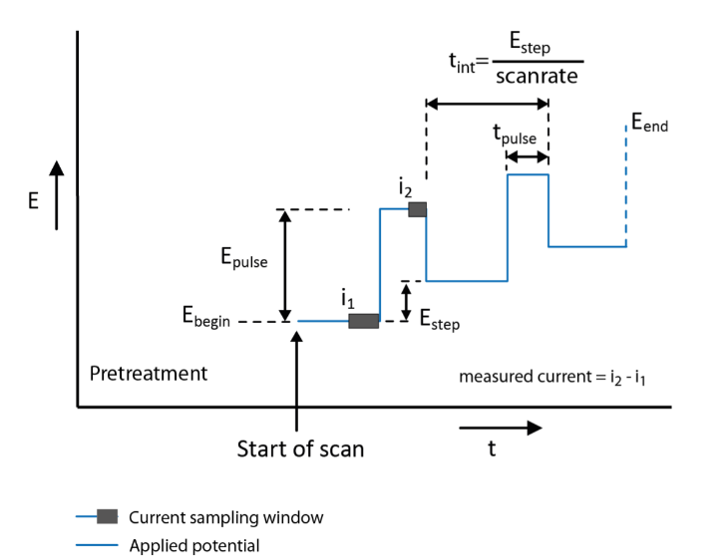
\includegraphics[width=0.7\linewidth]{figures/pulse.png}
    \caption{The \ac{DPV} excitation waveform, showing the staircase ramp, superimposed pulses, and the two current-sampling instants ($I_{\text{before}}$ and $I_{\text{end}}$) per step. }
    \label{fig:dpv_waveform}
\end{figure}

\mysubsection{Why DPV improves sensitivity}{Why DPV Improves Sensitivity / Reduces Background (Capacitive) Current Compared to LSV/CV}
\label{sec:dpv_sensitivity}

When a changing voltage occurs ($dV/dt$) over a brief period, a large spike in capacitive charging current occurs at the electrode-electrolyte interface. In continuous voltage sweeps such as CV or LSV, this capacitive noise is always present. The capacitive charging current decays exponentially as $e^{-t/RC}$, whereas the faradaic current decays much more slowly and is governed by the Cottrell equation, $1/\sqrt{t}$. To combat this, the second current measurement is taken at the end of the pulse width; this allows the double-layer capacitor time to fully charge so that the capacitive noise has died out, leaving only the faradaic signal. The resulting measurement has a much higher \ac{SNR}, allowing for the detection of much lower analyte concentrations. Analytes of interest span a large range of applications.

\mysubsection{Typical analytical applications}{Typical Analytical Applications (Trace Metals, Pharmaceuticals, Biosensing)}
\label{sec:dpv_applications}

Because \ac{DPV} effectively filters out capacitive charging current, it achieves exceptional sensitivity and low limits of detection, making it a foundational technique across multiple analytical fields. In environmental monitoring, DPV is frequently used in tandem with anodic stripping methods to detect trace heavy metals, such as lead and arsenic, at parts-per-billion concentrations in water systems. Within the pharmaceutical industry, it is used to analyse the purity of drug formulations and to study the oxidation mechanisms of active pharmaceutical ingredients. Furthermore, DPV is increasingly critical in the development of modern electrochemical biosensors. The biological fluids analysed in these systems (e.g.\ food or interstitial fluid) are highly resistive and generate significant background noise; by mathematically rejecting this noise, DPV allows microfluidic lab-on-a-chip devices to isolate the minute faradaic currents produced by specific biomarkers, enabling rapid and highly sensitive point-of-care diagnostics. All of these applications are controlled by a potentiostat.

\mysection{Potentiostat fundamentals}{Potentiostat Fundamentals}
\label{sec:potentiostat_fundamentals}

This section explores the fundamentals of a potentiostat, namely its role, design, performance parameters, and implementation approaches.

\mysubsection{The role of a potentiostat}{The Role of a Potentiostat}
\label{sec:role_potentiostat}

The role of a potentiostat is to control the control amplifier and the current-to-voltage amplifier (\ac{TIA}), and to buffer the reference electrode. For reference electrode buffering, the electrode must remain perfectly stable at a known half-cell potential; to prevent the voltage from drifting, zero current is allowed to flow through the electrode. This is achieved using an electrometer, an operational amplifier with an extremely high input impedance.

The control amplifier drives the system by constantly comparing the desired input voltage, set by a \ac{DAC}, with the actual voltage measured at the reference electrode. The resulting error signal is minimised by forcing current through the counter electrode and into the solution, which actively compensates for any changes in the electrochemical cell's resistance. The current-to-voltage converter (TIA) holds the working electrode at a 0\,V reference (virtual ground) while catching every electron produced or consumed by the reaction. These electrons generate a small faradaic current that is converted into a potential, which can then be measured by an \ac{ADC} \cite{bard2001}. Each of the three amplifiers is connected to one of the three electrodes.

\mysubsection{The classic 3-op-amp potentiostat topology}{The Classic 3-Operational Amplifier Potentiostat Topology}
\label{sec:3opamp_topology}

This section translates the three roles above into a physical circuit architecture, shown in Figure~\ref{fig:3opamp}.

\begin{itemize}
    \item \textbf{The feedback loop:} The 3-op-amp topology forms a negative feedback loop. The electrochemical cell itself (between the \ac{CE} and \ac{RE}) is physically placed inside the feedback path of the control amplifier.
    \item \textbf{Op-amp A (the driver):} The control amplifier.
    \item \textbf{Op-amp B (the buffer):} The RE voltage follower.
    \item \textbf{Op-amp C (the sensor):} The TIA connected to the WE.
\end{itemize}

\begin{figure}[H]
    \centering
    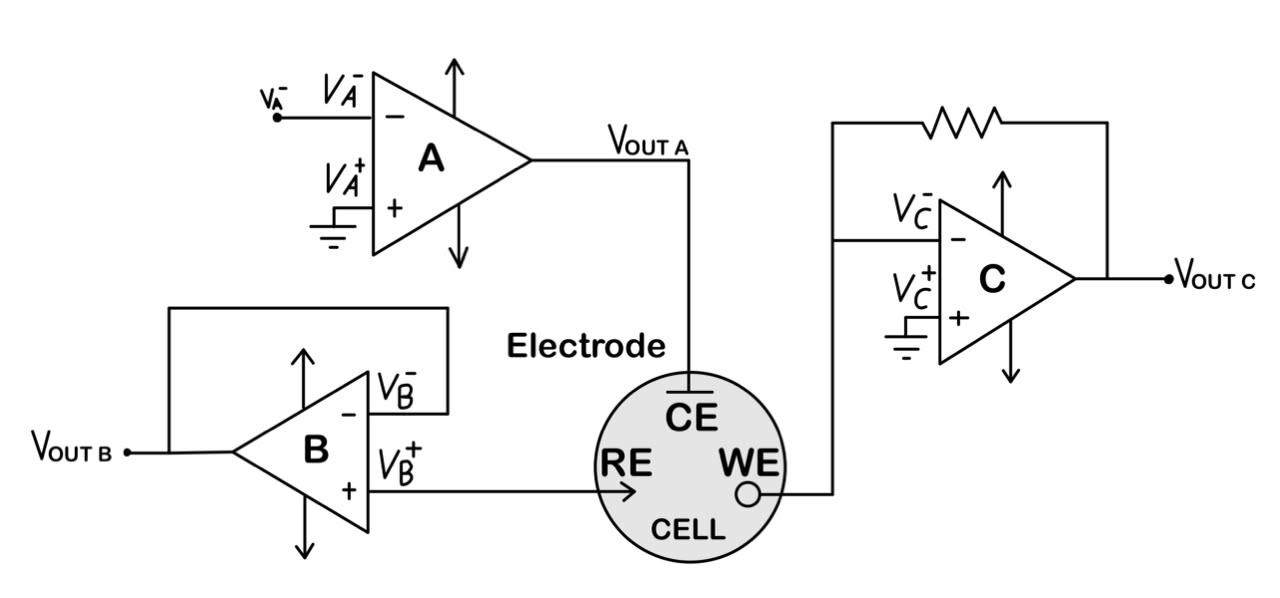
\includegraphics[width=0.7\linewidth]{figures/3opamp.jpeg}
    \caption{The classic 3-operational-amplifier potentiostat topology, showing the control amplifier, RE buffer, and TIA connected to the three electrodes.}
    \label{fig:3opamp}
\end{figure}

\mysubsection{Key performance parameters}{Key Performance Parameters}
\label{sec:key_performance_parameters}

This section establishes the criteria used to evaluate the effectiveness of the hardware, namely current measurement range and resolution, compliance voltage, noise floor, bandwidth, and technique support.

\begin{itemize}
    \item \textbf{Current measurement range and resolution:} In microfluidic biosensing, very small faradaic signals are generated. The potentiostat must be able to accurately measure down to the nanoampere (nA) or picoampere (pA) range without clipping or saturating the signal.

    \item \textbf{Compliance voltage:} This is the maximum voltage the control amplifier can physically output. Compliance voltage describes the ability of a power supply to push a much higher maximum voltage in order to keep a steady current flowing through a high-resistance load. If a fluid sample has high electrical resistance, the control amplifier needs a high compliance voltage to push the necessary current through the counter electrode.

    \item \textbf{Noise floor and \ac{LOD}:} The LOD of an electrochemical biosensor is fundamentally constrained by the inherent noise floor of the potentiostat's analog front end. In high-sensitivity applications, the TIA requires large feedback resistors to convert picoampere-level faradaic currents into measurable voltages. However, these resistive components inherently generate thermal (Johnson--Nyquist) noise, which scales with resistance and temperature. Therefore, a microfluidic diagnostic device targeting trace biomarkers (generating nanoampere or picoampere signals) requires a potentiostat topology with an exceptionally low electrical noise floor. If the peak-to-peak amplitude of the circuit's electronic noise exceeds the faradaic signal generated by the biomarker, reliable detection is physically impossible.

    \item \textbf{Bandwidth / scan rate limits:} This is the maximum speed at which the potentiostat can alter the applied potential. Fast techniques such as \ac{SWV} require high-bandwidth operational amplifiers to avoid signal distortion.

    \item \textbf{Technique support:} A system's ability to run CV, DPV, or \ac{EIS} depends on its \ac{DAC} resolution and internal waveform generators \cite{cruz2020}.
\end{itemize}

\mysubsection{Analog front-end approaches}{Analog Front-End Approaches}
\label{sec:afe_approaches}

Transitioning from the theoretical 3-op-amp topology to a physical implementation requires selecting an appropriate hardware architecture. While commercial benchtop potentiostats offer uncompromising analytical performance, their bulky form factors and high costs render them unsuitable for portable or point-of-care microfluidic diagnostics. Consequently, engineers developing custom electrochemical systems typically choose between two primary \ac{AFE} strategies: constructing a discrete circuit using individual operational amplifiers, or utilising a fully integrated \ac{SoC} AFE, such as the AD5941. Each approach presents distinct engineering trade-offs regarding power consumption, physical footprint, and architectural flexibility, which are summarised in Table~\ref{tab:afe_approaches}.

\begin{table}[H]
    \caption{Comparison of discrete op-amp and integrated AFE IC implementation approaches.}
    \footnotesize
    \centering
    \begin{tabular}{p{4cm}p{5cm}p{5cm}}
    \toprule
        \textbf{Implementation Approach} & \textbf{Advantages} & \textbf{Trade-offs} \\
    \midrule
        Discrete op-amp design &
        Unlimited architectural flexibility; capable of massive compliance voltages; component-level tuning for extreme precision &
        Large physical PCB footprint; high power consumption; complex board-level noise routing; higher cost of materials \\
        \addlinespace
        Integrated AFE ICs &
        Millimeter-scale physical footprint; ultra-low power consumption for \ac{IoT}; built-in hardware digital filtering; significantly lower per-unit cost &
        Hard-capped compliance voltage ($\leq 3$\,V); fixed internal current measurement ranges; black-box topology limits deep customisation; requires complex SPI/I2C firmware development \\
    \bottomrule
    \end{tabular}
    \label{tab:afe_approaches}
\end{table}

\mysection{Survey of existing potentiostat designs}{Survey of Existing Potentiostat Designs}
\label{sec:survey_designs}

The democratisation of electrochemical instrumentation has led to a rapid expansion of custom potentiostat designs. This section surveys the architectural evolution of these devices, establishing a performance baseline and identifying existing gaps in standalone usability and embedded intelligence.

\mysubsection{Commercial instruments}{Commercial Instruments}
\label{sec:commercial_instruments}

Commercial systems, such as the PalmSens EmStat or Metrohm Autolab, serve as the gold standard for electrochemical analysis. They offer uncompromising precision, massive dynamic ranges (pA to mA), rigorous factory calibration, and robust proprietary software suites. These instruments fall short in that they are cost-prohibitive (often exceeding thousands of dollars), physically bulky, and operate as closed-source devices, making them impossible to integrate deeply into custom, low-cost microfluidic or \ac{IoT} architectures. Nevertheless, they are exceedingly valuable in that they provide the foundational performance benchmarks against which all open-source and custom hardware must be validated \cite{palmsens2023}.

\mysubsection{Early open-source designs}{Early Open-Source Designs}
\label{sec:early_opensource}

The inception of open-source electrochemistry was marked by devices like the CheapStat \cite{rowe2011}. These devices proved that rudimentary analytical electrochemistry could be achieved with a \ac{BOM} under \$100, dramatically lowering the barrier to entry for educational and resource-limited settings. Since these first-generation potentiostats were built on early 8-bit microcontrollers, they suffered from poor \ac{ADC}/\ac{DAC} resolution, narrow voltage compliance windows, and a lack of wireless connectivity. CheapStat pioneered the open-hardware movement in electrochemistry, establishing the viability of DIY discrete op-amp topologies \cite{rowe2011}.

\mysubsection{General-purpose / high-performance open-source designs}{General-Purpose / High-Performance Open-Source Designs}
\label{sec:general_purpose_opensource}

To bridge the performance gap between early DIY builds and commercial units, high-performance open-source designs such as the DStat \cite{dryden2015} were developed. The DStat drastically improved noise performance, offered multi-technique support (CV, SWV, DPV, CA), and provided an excellent Python-based \ac{GUI}. Unfortunately, it remains tethered to a PC via USB for power and data processing; while highly accurate, this reliance on an external computer negates true field portability. This was the first time that custom discrete analog front-ends could achieve near-commercial sensitivity limits \cite{dryden2015}.

\mysubsection{Portable / wireless / smartphone-integrated designs}{Portable / Wireless / Smartphone-Integrated Designs}
\label{sec:portable_wireless}

The development of \ac{BLE} led to a generation of smartphone-integrated devices, such as the UWED and various ESP32-based We-VoltamoStat iterations \cite{ainla2018}. These devices achieved true field portability by offloading the processing and display requirements onto the user's smartphone, reducing the hardware footprint of the potentiostat itself. However, these designs are locked into their companion application: if the proprietary application is not maintained to support operating system updates, the hardware becomes obsolete \cite{ainla2018}. Furthermore, Bluetooth pairing can be unreliable in electrically noisy industrial environments \cite{automationworld_bluetooth}.

\mysubsection{EIS-capable / AFE-chip-based designs}{EIS-Capable / AFE-Chip-Based Designs}
\label{sec:eis_afe_designs}

The introduction of highly integrated, mixed-signal \acp{AFE} catalysed a shift away from bulky discrete op-amp circuits \cite{jenkins2019}. Systems like ABE-Stat, HunStat (2024), and HunStat2 (2025) characterise this generation. Utilising \acp{SoC} such as the AD5941 enables these devices to support complex, high-frequency techniques like \ac{EIS} while consuming fractions of a milliwatt; they boast exceptionally low electronic noise floors and millimeter-scale footprints \cite{hunstat2024,hunstat2_2025}. The development of ESP32 microcontrollers further aided performance as well as the appeal for DIY projects. However, the firmware required to configure the AFE registers is exceptionally complex, and devices such as HunStat are typically deployed as data-loggers; they lack built-in user interfaces and rely on raw serial data dumps for analysis. These two factors are an unfortunate downside of these systems \cite{hunstat2_2025}.

\mysubsection{Self-hosted web-interface / onboard-display designs}{Self-Hosted Web-Interface / Onboard-Display Designs}
\label{sec:selfhosted_webinterface}

To solve the challenge of being locked into a companion app, recent ESP32-based potentiostats have integrated embedded web servers. NanoStat \cite{lee2022} hosts an HTML5/JavaScript server, meaning any Wi-Fi-enabled device can control it via a standard browser. DM-Stat \cite{dmstat2024} and SaxStat \cite{saxstat2025} follow similar ``OpenEChem'' philosophies. A major benefit of this approach is ultimate cross-platform compatibility (Windows, macOS, iOS, Android) without requiring the user to install any software; however, hosting a web server consumes significant \ac{MCU} RAM and flash memory \cite{lee2022}.

There is a potential novelty gap in including a physical onboard display in such a system. A review of these systems reveals that they are almost exclusively headless. This highlights a distinct gap in the literature: a dual-interface approach would allow for rapid, standalone field testing without requiring the user to reach for a smartphone, while still preserving web-based data extraction capabilities.

\mysubsection{Machine-learning-assisted voltammetry}{Machine-Learning-Assisted Voltammetry}
\label{sec:ml_voltammetry}

The most recent paradigm shift involves embedding \ac{ML} algorithms directly onto the potentiostat's microcontroller. Examples include embedded multi-layer perceptrons for heavy-metal stripping voltammetry and models classifying \ac{DPV} responses for Dengue/Zika biomarkers on highly constrained hardware ($<$10\,kB RAM) \cite{mlheavymetal,mldengue}. Such models shift the system from mere data \textit{collection} to on-device data \textit{interpretation}, allowing the device to output actionable results (e.g.\ ``positive/negative'' or specific concentrations) rather than forcing a human expert to interpret a noisy voltammogram. These systems are less attractive in that they require extensive prior data collection to train the models, and inference algorithms consume heavy compute cycles on standard MCUs.

Table~\ref{tab:design_comparison} summarises the surveyed designs against the proposed architecture for this project.

\begin{table}[H]
    \caption{Comparison of surveyed potentiostat designs against the proposed architecture.}
    \tiny
    \centering
    \begin{tabular}{
        >{\raggedright\arraybackslash}p{2.3cm}
        >{\raggedright\arraybackslash}p{2.3cm}
        >{\raggedright\arraybackslash}p{2.6cm}
        >{\raggedright\arraybackslash}p{2.3cm}
        >{\raggedright\arraybackslash}p{1.5cm}
        >{\raggedright\arraybackslash}p{1.5cm}
        >{\raggedright\arraybackslash}p{2cm}
    }
    \toprule
        \textbf{Design / Platform} & \textbf{MCU / AFE Architecture} & \textbf{Primary Techniques Supported} & \textbf{Connectivity \& Interface} & \textbf{Onboard Display?} & \textbf{ML / Onboard Analysis?} & \textbf{Open-Source Completeness} \\
    \midrule
        Commercial (e.g.\ EmStat) & Proprietary & CV, DPV, SWV, EIS, CA & USB / Proprietary PC GUI & No & No (PC-based) & Closed source \\
        CheapStat (2011) & Atmel AVR / Discrete & CV, SWV, CA & None / Basic LCD output & Yes (Basic LCD) & No & Full (PCB/Firmware) \\
        DStat (2015) & Atmel XMEGA / Discrete & CV, DPV, SWV, CA & USB / Python PC GUI & No & No & Full (PCB/Firmware/GUI) \\
        Smartphone-Integrated (e.g.\ UWED) & BLE MCU / Discrete & CV, DPV, SWV & Bluetooth / Custom App & No & No & Partial (Hardware focus) \\
        HunStat2 (2025) & Mixed / AD5941 SoC & CV, DPV, SWV, EIS & USB / Serial Datalogging & No & No & Full (Hardware/Firmware) \\
        NanoStat (2022) & ESP32 / Discrete & CV, SWV, CA & Wi-Fi / Embedded Web GUI & No (Headless) & No & Full (Hardware/Web GUI) \\
        \textbf{Proposed ML Architecture} & ESP32 / AD5941 SoC & CV, DPV, SWV & Wi-Fi Web GUI + Standalone & Yes & Yes (Edge ML) & TBD \\
    \bottomrule
    \end{tabular}
    \label{tab:design_comparison}
\end{table}
